% ===================================================================
%  Week 9 — Lecture Notes (Persian) — Contours & Shape Analysis
% ===================================================================
\documentclass[12pt,a4paper]{article}
% ===================================================================
%  Shared preamble for Persian lecture notes (Image Processing).
%  Compile with XeLaTeX.  Body = Persian (RTL), code/math = LTR.
% ===================================================================

\usepackage{geometry}
\geometry{a4paper,margin=2.4cm}
\usepackage{amsmath,amssymb}
\usepackage{graphicx}
\usepackage{xcolor}
\usepackage{listings}
\usepackage{tcolorbox}
\usepackage{booktabs}
\usepackage{array}
\usepackage{enumitem}
\usepackage{hyperref}
\tcbuselibrary{skins,breakable}

% ---- Persian / RTL --------------------------------------------------
\usepackage{xepersian}
\settextfont{IRNazli}
\setlatintextfont{Latin Modern Roman}
\setdigitfont{IRNazli}
% More generous leading + paragraph spacing (Persian reads better with air).
\linespread{1.5}
\setlength{\parskip}{0.7em}

% ---- Colours --------------------------------------------------------
\definecolor{coursePrimary}{HTML}{1B4965}
\definecolor{courseAccent}{HTML}{E76F51}
\definecolor{courseGood}{HTML}{2A9D8F}
\definecolor{courseBad}{HTML}{C0392B}
\definecolor{courseInfo}{HTML}{2980B9}
\definecolor{codeBg}{HTML}{F5F6FA}
\definecolor{codeKw}{HTML}{8E44AD}
\definecolor{codeStr}{HTML}{2A9D8F}
\definecolor{codeCom}{HTML}{7F8C8D}

\hypersetup{colorlinks=true,linkcolor=courseInfo,urlcolor=courseInfo,citecolor=courseInfo}

% ---- Code listings (Python built in) -------------------------------
\lstdefinestyle{course}{
  backgroundcolor=\color{codeBg},
  basicstyle=\ttfamily\small,
  keywordstyle=\color{codeKw}\bfseries,
  stringstyle=\color{codeStr},
  commentstyle=\color{codeCom}\itshape,
  numberstyle=\tiny\color{codeCom},
  numbers=left, numbersep=7pt,
  showstringspaces=false, breaklines=true,
  tabsize=4, columns=fullflexible, frame=single,
  rulecolor=\color{gray!30}, keepspaces=true, upquote=true, language=Python,
}
\lstset{style=course}
\lstdefinelanguage{bash}{
  keywords={cd,pip,python,venv,source,import}, sensitive=true,
  morecomment=[l]{\#}, morestring=[b]', morestring=[b]",
}
\newenvironment{ltrcode}{\begin{LTR}}{\end{LTR}}

% ---- Callout boxes (Persian titles) --------------------------------
\newtcolorbox{yaddasht}{colback=courseInfo!8,colframe=courseInfo,
  title={\textbf{یادداشت}},boxrule=0.6pt,right=6pt,left=6pt,breakable}
\newtcolorbox{nokte}{colback=courseAccent!10,colframe=courseAccent,
  title={\textbf{نکتهٔ کلیدی}},boxrule=0.6pt,right=6pt,left=6pt,breakable}
\newtcolorbox{hoshdar}{colback=courseBad!8,colframe=courseBad,
  title={\textbf{هشدار / دام}},boxrule=0.6pt,right=6pt,left=6pt,breakable}
\newtcolorbox{riyazi}{colback=coursePrimary!6,colframe=coursePrimary,
  title={\textbf{ریاضیات}},boxrule=0.6pt,right=6pt,left=6pt,breakable}
\newtcolorbox{tamrin}{colback=courseGood!8,colframe=courseGood,
  title={\textbf{تمرین}},boxrule=0.6pt,right=6pt,left=6pt,breakable}

% ---- Header helper --------------------------------------------------
\newcommand{\coursemeta}[2]{%
  \begin{center}
  {\large\textbf{پردازش تصویرِ کاربردی}}\\[2pt]
  {\color{coursePrimary}\rule{\linewidth}{1pt}}\\[4pt]
  {\Large\textbf{#1}}\\[3pt]
  {\small جزوهٔ درس — #2}
  \end{center}\vspace{4pt}
}


\begin{document}
\coursemeta{جلسهٔ ۹ — کانتور، مؤلفه‌ها و تحلیلِ شکل}{هفتهٔ نهم}

{\small\itshape مکملِ اسلایدهای انگلیسیِ جلسهٔ ۹. تصاویر از کنتورِ واقعیِ شما تولید شده‌اند. هدف: کانتورها (طرحِ نواحی) و اندازه‌گیریِ شکل — مساحت، محیط، کادر، و توصیف‌گرها.}

\vspace{0.5cm}
\tableofcontents
\vspace{1cm}

% ===================================================================
\section{چرا این جلسه}

جلسهٔ ۸ نواحیِ جداشده داد. امروز \textbf{کانتور}‌ها — طرحِ کلیِ آن نواحی — و نحوهٔ \textbf{اندازه‌گیریِ}
شکل را یاد می‌گیریم. برای DocScan: کانتورِ هر رقم را بیابید، با کادرش برش دهید، و ارقام را مرتب
کنید — آخرین گام پیش از خواندن (جلسهٔ ۱۳).

\begin{nokte}
این جلسه پلِ نهاییِ «پیکسل به شیء» است. پس از این، هر رقم یک تصویرِ منزوی و مرتب‌شده است که آمادهٔ
شناسایی است. کیفیتِ یافتن و مرتب‌سازیِ کانتورها، مستقیماً عددِ نهاییِ خوانده‌شده را تعیین می‌کند.
\end{nokte}

\subsection{چرا شکل مهم است}

تا اینجا با \emph{شدت} (پیکسل‌ها) و \emph{نواحی} کار کردیم. اما بسیاری از تصمیم‌ها به \emph{شکل}
نیاز دارند: آیا این یک رقم است یا یک لکه؟ آیا این قطعه سالم است یا معیوب؟ آیا این سلول گرد است یا
کشیده؟ شکل، اطلاعاتی حمل می‌کند که شدتِ خام ندارد — و اغلب در برابرِ تغییرِ نور و رنگ مقاوم‌تر است.

تحلیلِ شکل، پیکسل‌ها را به \emph{ویژگی‌های عددی} (مساحت، گِردی، نسبتِ ابعاد) تبدیل می‌کند که
می‌توان با آن‌ها منطق ساخت: «اگر گِرد و کوچک است، یک سکه است»؛ «اگر بلند و باریک است، یک خراش
است، نه رقم». این پلِ بینِ «دیدن» و «فهمیدن» است.

\begin{nokte}
یک بینشِ کلیدی: خوبیِ تحلیلِ شکل کاملاً به کیفیتِ قطعه‌بندی و پاک‌سازیِ قبلی بستگی دارد. اگر ماسکِ
باینری تمیز باشد (جلسات ۷–۸)، تحلیلِ شکل ساده و دقیق است؛ اگر پُر از نویز و شکاف باشد، حتی
بهترین توصیف‌گرها هم بی‌فایده‌اند. برای همین این جلسه \emph{پس} از قطعه‌بندی و مورفولوژی می‌آید.
\end{nokte}

% ===================================================================
\section{یافتنِ کانتور}

یک \textbf{کانتور} فهرستِ مرتبی از نقاطِ مرزیِ یک ناحیهٔ سفیدِ همبند است. از یک تصویرِ باینریِ تمیز،
\lr{findContours} طرحِ هر شیء را ردیابی می‌کند.

\begin{center}

\includegraphics[width=0.44\linewidth]{../assets/binary.png}\quad
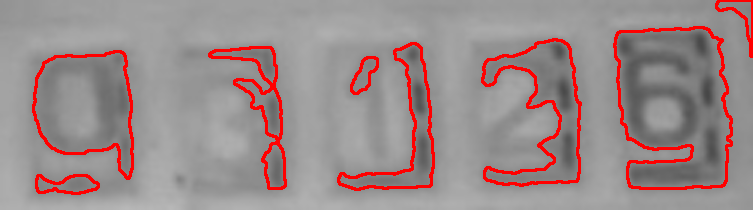
\includegraphics[width=0.44\linewidth]{../assets/contours.png}\\[2pt]
{\small چپ: ارقامِ باینری — راست: کانتورها (قرمز)}
\end{center}

\begin{ltrcode}
\begin{lstlisting}[language=Python]
contours, hierarchy = cv2.findContours(binary,
    cv2.RETR_EXTERNAL,        # only outer contours (ignore holes)
    cv2.CHAIN_APPROX_SIMPLE)  # compress straight segments to endpoints
\end{lstlisting}
\end{ltrcode}

\begin{itemize}
  \item \lr{RETR\_EXTERNAL}: فقط مرزهای بیرونی. \lr{RETR\_TREE}: سلسله‌مراتبِ کاملِ تودرتویی.
  \item \lr{CHAIN\_APPROX\_SIMPLE}: فقط نقاطِ گوشه را ذخیره می‌کند (یک مستطیل = ۴ نقطه، نه صدها).
\end{itemize}

\subsection{حالت‌های بازیابیِ کانتور}

\lr{findContours} حالت‌های مختلفی دارد که چه کانتورهایی و با چه ساختاری برگردانده شوند:

\begin{center}
\begin{tabular}{>{\raggedright\arraybackslash}p{0.3\linewidth} >{\raggedright\arraybackslash}p{0.6\linewidth}}
\toprule
\textbf{حالت} & \textbf{رفتار} \\
\midrule
\lr{RETR\_EXTERNAL} & فقط کانتورهای بیرونی (رایج‌ترین برای برشِ اشیا) \\
\lr{RETR\_LIST} & همهٔ کانتورها، بدونِ سلسله‌مراتب \\
\lr{RETR\_CCOMP} & دو سطح: بیرونی و سوراخ‌ها \\
\lr{RETR\_TREE} & سلسله‌مراتبِ کاملِ تودرتویی \\
\bottomrule
\end{tabular}
\end{center}

\textbf{سلسله‌مراتب} (\lr{hierarchy}) می‌گوید کدام کانتور درونِ کدام است. مثال: یک رقمِ «۰» یک
کانتورِ بیرونی و یک کانتورِ درونی (سوراخ) دارد. شمردنِ سوراخ‌ها یک ویژگیِ ارزان است: «۰»، «۶»،
«۸»، «۹» سوراخ دارند؛ «۱»، «۲»، «۳»، «۵»، «۷» ندارند. این می‌تواند به تفکیکِ اولیهٔ ارقام کمک کند.

\subsection{کانتور در برابرِ مؤلفهٔ همبند}

\textbf{مؤلفه‌های همبند} هر پیکسل را با شناسهٔ ناحیه‌اش برچسب می‌زنند (یک تصویرِ برچسب‌خورده).
\textbf{کانتورها} \emph{مرزِ} مرتبِ هر ناحیه را می‌دهند (فهرستی از نقاط). از مؤلفه‌ها برای
شمارش/برچسب، از کانتورها برای اندازه‌گیریِ شکل و برش استفاده کنید. اغلب با هم به کار می‌روند: هر
دو یک ماسکِ باینری را به فهرستی از اشیا تبدیل می‌کنند — پلِ پیکسل به چیزهای قابلِ‌شمارش و اندازه‌گیری.

% ===================================================================
\section{اندازه‌گیریِ شکل}

\begin{center}
\begin{tabular}{>{\raggedright\arraybackslash}p{0.4\linewidth} >{\raggedright\arraybackslash}p{0.5\linewidth}}
\toprule
\textbf{اندازه‌گیری} & \textbf{OpenCV} \\
\midrule
مساحت & \lr{cv2.contourArea(c)} \\
محیط & \lr{cv2.arcLength(c, True)} \\
کادرِ محوری & \lr{cv2.boundingRect(c)} \\
کادرِ چرخیده & \lr{cv2.minAreaRect(c)} \\
دایرهٔ محیطی & \lr{cv2.minEnclosingCircle(c)} \\
مرکزِ ثقل & از \lr{cv2.moments(c)} \\
\bottomrule
\end{tabular}
\end{center}

این‌ها شکل را به اعدادی تبدیل می‌کنند که می‌توانید فیلتر، مرتب و مقایسه کنید.

\subsection{کادر $\rightarrow$ برش و مرتب‌سازیِ ارقام}

\begin{center}
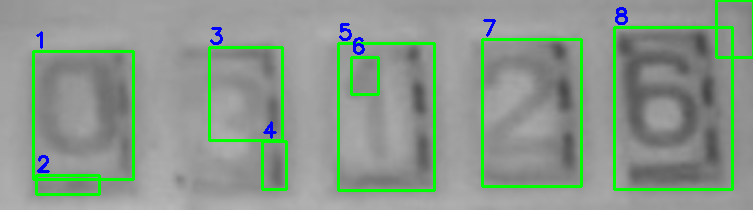
\includegraphics[width=0.85\linewidth]{../assets/boxes.png}\\[2pt]
{\small کادرِ هر رقم، شماره‌گذاری‌شده چپ‌به‌راست}
\end{center}

دورِ هر رقم یک کادر بکشید؛ کادرها را بر اساسِ مختصاتِ $x$ (چپ‌به‌راست) مرتب کنید. هر کادر را برش
دهید $\rightarrow$ یک تصویرِ تمیز به‌ازای هر رقم، \emph{به ترتیب}. این دقیقاً تحویلِ DocScan به
شناسایی‌گر (جلسهٔ ۱۳) است.

\subsection{فیلترکردن بر اساسِ شکل}

تصاویرِ واقعی کانتورهای زائد می‌دهند (لکه‌های نویز، علائمِ ناقص). با این‌ها فیلتر کنید:
\textbf{مساحت} (خیلی کوچک = نویز)، \textbf{نسبتِ ابعاد} (ارقام بلندتر از پهنا)، \textbf{گستره} (کسرِ پُرشدگی).

\begin{nokte}
یک قاعدهٔ مقاوم: «کانتورها را با مساحتِ $>T$ و $0.2 < w/h < 1.2$ نگه دار» — چون ارقام جمع‌وجور و
نسبتاً بلندند. چند آستانهٔ ساده، بیشترِ مثبت‌های کاذب را حذف می‌کند.
\end{nokte}

\subsection{پوستهٔ محدب و تحدب}

\begin{center}
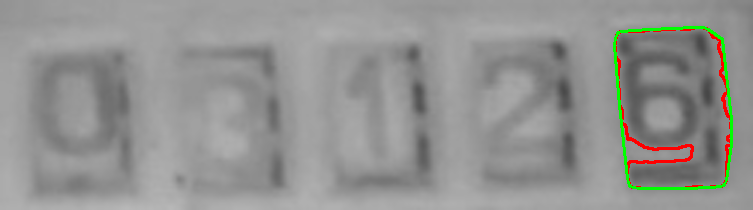
\includegraphics[width=0.5\linewidth]{../assets/hull.png}\\[2pt]
{\small کانتور (قرمز) + پوستهٔ محدب (سبز)}
\end{center}

\textbf{پوستهٔ محدب} (\lr{convex hull}): کوچک‌ترین شکلِ محدبی که کانتور را در بر می‌گیرد (یک کشِ
لاستیکی). \textbf{نقص‌های تحدب} (فرورفتگی‌ها) انگشت‌ها، شکاف‌ها، یا گردنِ اشیای چسبیده را آشکار
می‌کنند. \textbf{صلبیت} (\lr{solidity}) = مساحت / مساحتِ پوسته — چقدر شکل «پُر» است.

% ===================================================================
\section{توصیف‌گرهای شکل}

\begin{itemize}
  \item \textbf{گِردی} $= 4\pi\,\text{مساحت}/\text{محیط}^2$ (۱ برای دایره، کمتر برای شکل‌های پیچیده).
  \item \textbf{نسبتِ ابعاد}، \textbf{گستره} (مساحت/مساحتِ کادر)، \textbf{صلبیت} (مساحت/مساحتِ پوسته).
  \item \textbf{ممان‌ها} (\lr{moments}): جمع‌های وزن‌دار که یک شکل را خلاصه می‌کنند (مرکز، جهت، پراکندگی).
\end{itemize}

\begin{riyazi}
مرکزِ ثقل: $\bar{x}=M_{10}/M_{00}$، $\bar{y}=M_{01}/M_{00}$، که $M_{00}$ مساحت است. ممان‌های
مرتبهٔ بالاتر جهت و کشیدگیِ شکل را می‌دهند.
\end{riyazi}

\subsection{ممان‌های Hu: شکلِ مقاوم به چرخش/مقیاس}

\textbf{ممان‌های Hu}: ۷ عدد که (تقریباً) به \textbf{انتقال، چرخش و مقیاس} ناوردا هستند. پس همان
شکل، صرفِ‌نظر از کجا/چه‌قدر بزرگ/چرخیده، همان توصیف‌گر را می‌دهد. مفید برای تطبیقِ یک شکل با یک
الگو — جایگزینِ کلاسیکِ یک شبکهٔ عصبی. \lr{cv2.matchShapes} دو کانتور را با ممان‌های Hu مقایسه
می‌کند — یک امتیازِ شباهتِ سریع.

\subsection{مثالِ عددیِ توصیف‌گرها}

بیایید چند توصیف‌گر را برای دو شکل حساب کنیم تا کاربردشان روشن شود. فرض کنید یک رقمِ «۱» و یک لکهٔ
نویز داریم:

\textbf{رقمِ «۱»}: مساحت ۳۰۰ پیکسل، کادر $10 \times 40$ (پهنا×بلندی). نسبتِ ابعاد $= 10/40 = 0.25$
(بلند و باریک)؛ گستره $= 300/(10 \times 40) = 0.75$ (کادر را خوب پُر می‌کند).

\textbf{لکهٔ نویز}: مساحت ۱۵ پیکسل، کادر $4 \times 4$. نسبتِ ابعاد $= 1.0$ (مربعی)؛ مساحتِ خیلی کوچک.

با این اعداد، یک فیلترِ ساده «مساحت > ۱۰۰ و نسبتِ ابعاد < ۰٫۸» رقم را نگه و لکه را حذف می‌کند.
دیدید که چطور چند توصیف‌گرِ عددی، تصمیمِ «رقم یا نویز» را ممکن می‌کنند؟ این قدرتِ تحلیلِ شکل است:
تبدیلِ یک قضاوتِ بصری به یک قاعدهٔ عددیِ قابلِ‌کدنویسی.

\subsection{تقریبِ کانتور (برازشِ چندضلعی)}

\lr{approxPolyDP} یک کانتور را به نقاطِ کمتر (در یک تلورانس) ساده می‌کند. مرزِ یک صفحه/سند
$\rightarrow$ به \emph{۴ نقطه} = گوشه‌ها تقریب می‌زند. آن ۴ گوشه، تصحیحِ پرسپکتیوِ جلسهٔ ۱۱ را
تغذیه می‌کنند — گامِ «صاف‌کردن»ِ DocScan.

\begin{nokte}
تقریبِ کانتورِ صفحه به یک چهارضلعی، همان راهی است که DocScan گوشه‌های صفحه را می‌یابد. این نمونهٔ
زیبایی از استفاده از تحلیلِ شکل برای یک هدفِ کاملاً عملی است.
\end{nokte}

% ===================================================================
\section{ممان‌ها با جزئیات}

ممان‌ها ابزارِ ریاضیِ قدرتمندی برای توصیفِ شکل‌اند. ممانِ خامِ مرتبهٔ $(p, q)$ چنین تعریف می‌شود:

\begin{riyazi}
$M_{pq} = \sum_x \sum_y x^p\, y^q\, I(x,y)$
\end{riyazi}

از این‌ها اطلاعاتِ مفید استخراج می‌شود: $M_{00}$ = مساحت (مجموعِ پیکسل‌ها)؛ $M_{10}/M_{00}$ و
$M_{01}/M_{00}$ = مرکزِ ثقل. \textbf{ممان‌های مرکزی} (نسبت به مرکزِ ثقل) به انتقال ناوردا هستند، و
با نرمال‌سازی به مقیاس هم ناوردا می‌شوند. ممان‌های Hu ترکیب‌های خاصی از این‌ها هستند که علاوه بر
این به \emph{چرخش} هم ناوردایند.

\begin{nokte}
چرا ناوردایی مهم است؟ چون یک رقمِ «۷» باید همان توصیف‌گر را بدهد چه کوچک چه بزرگ، چه صاف چه کمی
کج. یک توصیف‌گرِ ناوردا، تطبیق و دسته‌بندی را در برابرِ این تغییرات مقاوم می‌کند — همان چیزی که یک
CNN هم باید یاد بگیرد، اما ما اینجا آن را از ریاضی می‌سازیم.
\end{nokte}

% ===================================================================
\section{زنجیرهٔ کد و بازنماییِ مرز}

یک راهِ فشرده برای ذخیرهٔ کانتور، \textbf{زنجیرهٔ کد} (\lr{chain code}) است: به‌جای ذخیرهٔ مختصاتِ
هر نقطه، فقط \emph{جهتِ} حرکت به نقطهٔ بعدی را ذخیره می‌کنید (۸ جهتِ ممکن، هرکدام یک رقم). این
بازنمایی فشرده است و ویژگی‌های جالبی دارد: چرخشِ ۹۰ درجه فقط اعداد را جابه‌جا می‌کند، و می‌توان از
آن ویژگی‌های ناوردا استخراج کرد.

\lr{CHAIN\_APPROX\_SIMPLE} که در کد استفاده کردیم، یک بهینه‌سازیِ مرتبط است: به‌جای ذخیرهٔ هر
پیکسلِ روی یک خطِ راست، فقط دو نقطهٔ انتهایی را نگه می‌دارد. برای یک مستطیل، این یعنی ۴ نقطه به‌جای
صدها — صرفه‌جوییِ حافظه و سرعتِ چشمگیر.

\begin{yaddasht}
انتخابِ بازنماییِ درست برای یک کانتور — فهرستِ نقاط، زنجیرهٔ کد، توصیف‌گرِ فوریه، یا ممان — به هدف
بستگی دارد: ذخیره، تطبیق، یا اندازه‌گیری. هر بازنمایی مبادله‌ای بین فشردگی، ناوردایی، و سهولتِ
محاسبه دارد.
\end{yaddasht}

% ===================================================================
\section{تمرینِ کلاسیِ وسط‌جلسه (۱۲ دقیقه)}

\begin{tamrin}
از یک عکسِ کنتور کانتورهایی دارید: ۹ رقم به‌علاوهٔ چند لکهٔ نویز و یک خراشِ بلند. (۱) کدام
اندازه‌گیری‌ها یک رقم را از یک لکه متمایز می‌کنند؟ از یک خراش؟ (۲) یک قاعدهٔ فیلتر (مساحت + نسبتِ
ابعاد) بنویسید که ارقام را نگه دارد و بقیه را حذف کند. (۳) پس از فیلتر، عدد را چطور به ترتیبِ درست
خروجی می‌دهید؟
\end{tamrin}

\textbf{جمع‌بندی:} لکه: مساحتِ ریز $\rightarrow$ حذف با \lr{area > T}. خراش: نسبتِ ابعادِ حاد (خیلی
پهن/نازک) $\rightarrow$ حذف. قاعده: نگه دار اگر \lr{area>200 and 0.2<w/h<1.2} — ارقام جمع‌وجور و
بلندند. ترتیب: کادرهای نگه‌داشته را بر اساسِ $x$ مرتب کنید؛ چپ‌به‌راست بخوانید. اندازه‌گیریِ شکل،
«کدام لکه‌ها رقم‌اند؟» را به چند آستانهٔ عددی تبدیل می‌کند.

% ===================================================================
\section{بخشِ عمیق}

\subsection{شمارش و اندازه‌گیریِ اشیا}

شمارش = تعدادِ کانتورهای معتبر (پس از فیلتر) — سلول، سکه، قطعه، رقم. اندازه‌گیری = مساحت/طول/قطر
به‌ازای هر کانتور، تبدیل‌شده به واحدِ واقعی با یک مقیاسِ معلوم. این ستونِ فقراتِ بازرسیِ صنعتی و
میکروسکوپی است — بیناییِ کلاسیکِ محض. یک نسبتِ کالیبره‌شدهٔ پیکسل-به-میلی‌متر، اندازه‌گیریِ کانتور
را به ابعادِ دنیای واقعی تبدیل می‌کند.

\subsection{کالیبراسیون: از پیکسل به میلی‌متر}

اندازه‌گیریِ کانتور به پیکسل است، اما دنیای واقعی به میلی‌متر. برای تبدیل، یک \textbf{مرجعِ معلوم}
لازم است: یک شیء با اندازهٔ معلوم در تصویر (مثلِ یک سکه یا یک خط‌کش). اگر یک سکهٔ ۲ سانتی‌متری در
تصویر ۱۰۰ پیکسل قطر دارد، پس مقیاس ۰٫۰۲ سانتی‌متر بر پیکسل است، و می‌توانید هر اندازه‌گیریِ دیگر
را تبدیل کنید.

مثالِ عملی: اگر یک قطعهٔ صنعتی در تصویر مساحتِ ۵۰۰۰ پیکسلِ مربع دارد و مقیاس ۰٫۰۲ سانتی‌متر بر
پیکسل است، مساحتِ واقعی $= 5000 \times 0.02^2 = 2$ سانتی‌متر مربع. این تبدیل، تحلیلِ شکل را از یک
تمرینِ انتزاعی به یک ابزارِ اندازه‌گیریِ واقعی بدل می‌کند.

\begin{nokte}
کالیبراسیون یکی از مهم‌ترین گام‌ها در بیناییِ اندازه‌گیری است و اغلب نادیده گرفته می‌شود. بدونِ آن،
اعدادِ شما فقط «پیکسل» هستند، نه اندازه‌های معنادار. در بازرسیِ صنعتی، دقتِ کالیبراسیون مستقیماً
دقتِ اندازه‌گیری را تعیین می‌کند.
\end{nokte}

\subsection{مقاومت: آشوبِ کانتورِ دنیای واقعی}

کانتورها فقط به‌اندازهٔ ماسکِ باینری خوب‌اند — زباله داخل، زباله بیرون. رقمِ شکسته $\rightarrow$
دو کانتور؛ ارقامِ ادغام‌شده $\rightarrow$ یک کانتور. بالادست را رفع کنید (جلسات ۷–۸). همیشه بر
اساسِ شکل فیلتر کنید \emph{و} تعداد را روی دادهٔ واقعی بررسیِ سلامت کنید.

\begin{hoshdar}
تعدادِ کانتور را کورکورانه باور نکنید — یک سایه یا یک لکه می‌تواند شیء اضافه یا ادغام کند. برای
کنتور، اگر تعدادِ ارقام معلوم است (مثلاً همیشه ۵ رقم)، از آن به‌عنوانِ بررسیِ سلامت استفاده کنید.
\end{hoshdar}

\subsection{توصیف‌گرهای فوریه}

یک کانتور را به‌صورتِ یک سیگنال بازنمایی و تبدیلِ فوریه‌اش را بگیرید (جلسهٔ ۶ دوباره). ضرایبِ
فرکانس‌پایین = شکلِ کلی؛ بالا = جزئیاتِ ریزِ مرز. نگه‌داشتنِ چند ضریب، یک توصیف‌گرِ شکلِ فشرده و
مقاوم برای تطبیق می‌دهد.

\subsection{تطبیقِ شکل با matchShapes}

فرض کنید یک الگوی «شکلِ رقمِ ۷» دارید و می‌خواهید ببینید یک کانتورِ ناشناخته چقدر شبیهِ آن است.
\lr{cv2.matchShapes} ممان‌های Huِ دو کانتور را مقایسه و یک امتیازِ فاصله برمی‌گرداند (صفر = یکسان).
چون Hu به چرخش/مقیاس ناوردا است، این تطبیق حتی اگر رقم کمی چرخیده یا اندازه‌اش متفاوت باشد کار می‌کند.

\begin{ltrcode}
\begin{lstlisting}[language=Python]
score = cv2.matchShapes(template_contour, unknown_contour,
                        cv2.CONTOURS_MATCH_I1, 0.0)
# smaller score = more similar shape
\end{lstlisting}
\end{ltrcode}

این یک روشِ کلاسیکِ تشخیصِ شکل است: یک بانکِ الگو بسازید و هر کانتورِ ناشناخته را با همه مقایسه
کنید؛ نزدیک‌ترین الگو، دسته را می‌دهد. برای شکل‌های ساده و متمایز خوب کار می‌کند، اما برای ارقامِ
دست‌نویسِ متنوع، یک CNN (جلسهٔ ۱۳) بسیار دقیق‌تر است.

\subsection{الگوریتمِ ردیابیِ کانتور}

پشتِ \lr{findContours} یک الگوریتمِ کلاسیک (\lr{Suzuki-Abe}) است که مرزها را با «دنبال‌کردنِ»
پیکسل‌های مرزی ردیابی می‌کند: از یک پیکسلِ مرزی شروع، و در جهتِ ساعت‌گرد دورِ شیء حرکت می‌کند تا به
نقطهٔ شروع برگردد. همین حین، سلسله‌مراتب (کدام کانتور درونِ کدام) را هم می‌سازد. فهمِ اینکه این یک
ردیابیِ ساده است، به شما کمک می‌کند درک کنید چرا کانتورها همیشه \emph{بسته} و \emph{مرتب}‌اند —
ویژگی‌ای که برایِ اندازه‌گیری و برش حیاتی است.

\subsection{تحلیلِ شکل $\rightarrow$ شناسایی}

ممان‌های Hu/توصیف‌گرها می‌توانند شکل‌های ساده را بدونِ هیچ آموزشی دسته‌بندی کنند. برای ارقام،
توصیف‌گرهای دست‌ساز کار می‌کنند اما یک CNN (جلسهٔ ۱۳) دقیق‌تر است. خطِ لوله یکسان است: قطعه‌بندی
$\rightarrow$ کانتور/برش $\rightarrow$ توصیف/دسته‌بندی.

% ===================================================================
\section{این جلسه در پروژهٔ نهایی}

خطِ لولهٔ کاملِ استخراجِ رقم:

\begin{ltrcode}
\begin{lstlisting}[language=Python]
cnts, _ = cv2.findContours(binary, cv2.RETR_EXTERNAL, cv2.CHAIN_APPROX_SIMPLE)
digits = []
for c in cnts:
    x, y, w, h = cv2.boundingRect(c)
    if cv2.contourArea(c) > 200 and 0.2 < w/h < 1.2:   # keep digit-like
        digits.append((x, gray[y:y+h, x:x+w]))
digits = [img for x, img in sorted(digits)]            # left-to-right order
# each `img` is one digit, ready for the recognizer (Week 13)
\end{lstlisting}
\end{ltrcode}

\begin{yaddasht}
\textbf{مایلستونِ هفتهٔ ۹:} از یک عکسِ کنتور، یک تصویرِ برش‌خورده و مرتب‌شده به‌ازای هر رقم تولید
کنید. این خروجی مستقیماً ورودیِ شناساییِ جلسهٔ ۱۳ است. همچنین، برای بخشِ «یافتنِ صفحه»ی DocScan،
کانتورِ بیرونیِ سند را به ۴ گوشه تقریب بزنید (که در جلسهٔ ۱۱ برای صاف‌کردن استفاده می‌شود).
\end{yaddasht}

% ===================================================================
\section{جمع‌بندی}

\begin{itemize}
  \item یافتنِ کانتور؛ انتخابِ حالتِ بازیابی و تقریب.
  \item اندازه‌گیریِ مساحت/محیط/کادر/مرکز؛ محاسبهٔ توصیف‌گرهای شکل.
  \item فیلترکردنِ کانتور بر اساسِ شکل؛ استفاده از ممان‌های Hu برای تطبیقِ ناوردا.
  \item تقریبِ کانتورِ صفحه به ۴ گوشه؛ برش و مرتب‌سازیِ ارقام.
\end{itemize}

\begin{tamrin}
\textbf{تحویلیِ این هفته (پیش از جلسهٔ ۱۰):} (۱) کانتورها را روی یک باینریِ تمیزِ کنتور بیابید و
رسم کنید؛ مساحت و کادرِ هر رقم را گزارش دهید. (۲) کانتورهای نویز را با قاعدهٔ مساحت + نسبتِ ابعاد
حذف کنید؛ تعداد را بررسی کنید. (۳) هر رقم را با کادرش برش دهید و مرتب‌شده چپ‌به‌راست خروجی دهید.
(۴) امتیازی: کانتورِ بیرونیِ یک سند را به ۴ گوشه تقریب بزنید.
\end{tamrin}

\subsection*{کاربردهای تحلیلِ شکل}

\begin{itemize}
  \item \textbf{OCR}: جدا و آماده‌سازیِ هر کاراکتر (DocScan).
  \item \textbf{شمارش}: سلول، سکه، قطعه، دانه.
  \item \textbf{اندازه‌گیری}: ابعادِ قطعه در بازرسیِ صنعتی.
  \item \textbf{دسته‌بندیِ شکل}: تشخیصِ نوعِ شیء از توصیف‌گرها.
  \item \textbf{یافتنِ سند}: تقریبِ کانتور به چهارضلعی برای صاف‌کردن.
\end{itemize}

\subsection*{چک‌لیستِ دام‌های این هفته}

\begin{itemize}
  \item کانتور روی ماسکِ بد (زباله داخل، زباله بیرون) — اول باینریِ خوب.
  \item فراموشیِ فیلترِ شکل (کانتورهای نویز به‌عنوانِ رقم) — قاعدهٔ مساحت + نسبت.
  \item فراموشیِ مرتب‌سازی (ترتیبِ غلطِ رقم) — بر اساسِ $x$ مرتب کنید.
  \item انتظارِ ناوردایی از مساحت/محیط (که نیستند) — از ممان‌های Hu برای ناوردایی.
  \item باور کورکورانهٔ تعداد — بررسیِ سلامت با تعدادِ موردِ انتظار.
\end{itemize}

\subsection*{واژه‌نامهٔ کوتاه}

\begin{center}
\begin{tabular}{>{\raggedright\arraybackslash}p{0.3\linewidth} >{\raggedright\arraybackslash}p{0.6\linewidth}}
\toprule
\textbf{اصطلاح} & \textbf{معنی} \\
\midrule
\lr{Contour} & مرزِ مرتبِ یک ناحیه \\
\lr{Bounding box} & کادرِ محیطیِ یک شکل \\
\lr{Moments} & جمع‌های وزن‌دارِ توصیف‌کنندهٔ شکل \\
\lr{Hu moments} & ۷ توصیف‌گرِ ناوردا به چرخش/مقیاس \\
\lr{Convex hull} & کوچک‌ترین شکلِ محدبِ دربرگیرنده \\
\lr{approxPolyDP} & ساده‌سازیِ کانتور به چند نقطه \\
\bottomrule
\end{tabular}
\end{center}

\vspace{0.5cm}
\begin{center}
\textit{کانتورها نواحی را به اشیای قابلِ‌اندازه‌گیری تبدیل می‌کنند. بیاب، اندازه بگیر، فیلتر کن، برش بده، مرتب کن.}
\end{center}

\end{document}
